\documentclass{pre-tfg}

%\showhelp  % comenta o borra para eliminar ayudas

\usepackage{graphicx}

\title{SISTEMA DE CONTROL VISUAL EMPOTRADO UTILIZANDO FPGA PARA DETECCIÓN DE OBSTÁCULOS}
\author{José Jiménez Rincón}
\advisorFirst{Julio Daniel Dondo Gazzano}
\advisorDepartment{DEPARTAMENTO DE TECNOLOGIAS Y SISTEMAS DE INFORMACION}
\advisorSecond{}
\intensification{INGENIERÍA DE COMPUTADORES}
\docdate{2016}{Febrero}

\begin{document}

\maketitle
\tableofcontents

\newpage

%El anteproyecto recogería, en un \textcolor[rgb]{0.5,0.0,0.0}{máximo de 10 páginas},
%los siguientes apartados:
%
%\begin{itemize}
%\item Introducción (muy recomendable aunque no obligatorio)
%\item Tecnología específica cursada por el alumno
%\item Objetivos
%\item Método y fases de trabajo
%\item Medios que se pretenden utilizar
%\item Bibliografía básica consultada en la elaboración del anteproyecto
%\item Contrato de propiedad intelectual (si lo hubiera)
%\end{itemize}


\section{INTRODUCCIÓN}

%%%HECHO-NOTA1: 
% La introducción se puede mejorar indicando qué problema estamos atacando con esta idea o para que puede servir, por ejemplo para acceso a lugares remotos, utilizando hardware reconfigurable para mejorar y acelerar el procesamiento de imágenes en  tiempo real, etc. en lugar de contar como se te ocurrio o surgió la idea, (lo que es unicamente anecdótico). Creo que es mas profesional explicar cual es el problema que quieres solucionar. En cualquier caso he corregido lo que estaba.

%HECHO-OTRA COSA IMPORTANTE Buscar en internet acerca de los problemas existentes en la detección de obstáculos y el control de movimiento de robots, y agregarlo en la introducción.


%%RECUERDA ESTO QUE VIENE EN LA NORMATIVA

%El capítulo de introducción podrá abordar los siguientes aspectos:
%
%\begin{itemize}
%\item Introducción al tema, entorno en el que el trabajo desempeñará
%  su objetivo, justificación de la importancia del trabajo abordado.
%\item Motivación y antecedentes (con algunas referencias bibliográficas).
%\item Descripción gráfica del proyecto (es aconsejable incorporar una figura que describa
%  el trabajo a desarrollar y que mejore la comprensión del mismo).
%\end{itemize}

Esta propuesta de TFG surge de analizar la problemática existente de la utilización de hardware reconfigurable en el procesamiento de imágenes en tiempo real.

Debido a que el objetivo principal del proyecto es conseguir que un vehículo, mediante el uso de una cámara cenital, esquive los objetos en tiempo real hasta llegar a su destino. 

Este objetivo plantea tres problemas principales, según \cite{Problemas}, para que se pueda llevar a cabo:

\begin{itemize}
\item La correcta detección de obstáculos.
\item Técnicas para evitar colisiones 
\end{itemize}

Para realizar una correcta detección de obstáculos se deberá abordar la problemática de cómo distinguir los objetos que aparecen en una imagen del entorno en el que vamos a trabajar. Para ello, se deberá realizar un estudio del lugar en el que se van a realizar las pruebas, para ajustar los algoritmos de detección de obstáculos a los condicionantes principales del entorno. Como por ejemplo, la luminosidad, el tipo de objetos que queremos esquivar (distinguir el suelo frente a los objetos), ajustar la distancia en la que se va a colocar la cámara, etc... Ya que si se aplicaran los algoritmos estudiados para un entorno, en un entorno distinto, los resultados se verían notablemente afectados.

En lo referente a las técnicas para evitar colisiones surge un problema a la hora de calcular la trayectoria que debe seguir el vehículo, ya que, se debe controlar que la anchura de la trayectoria que se va a calcular permita el paso del vehículo. Mediante que para calcular la trayectoria, una vez hemos ajustado los parámetros de la anchura, podría utilizarse cualquiera de estos algoritmos de camino más corto:

\begin{itemize}
\item A*
\item Dijkstra
\item Viterbi
\end{itemize} 

Una vez se resuelvan estos dos principales problemas podremos conseguir objetivos tales como:

\begin{itemize}
\item Utilizar hardware reconfigurable para mejorar y acelerar el procesamiento de imágenes en tiempo real.
\item Acceder a lugares remotos mediante el uso de un vehículo dirigido por señales, generadas automáticamente por nuestro sistema. 
\item Desarrollar un sistema capaz de esquivar objetos en tiempo real mediante el uso de algoritmos de detección de bordes~\cite{Edges}.
\item Traducir las señales enviadas por la placa Zedboard de AVNET~\cite{Zedboard}, con FPGAs de la firma Xillinx~\cite{Fpga}, en movimientos que realizará el vehículo.
\end{itemize}


% HECHO-La descripción de un anteproyecto, o una memoria de un proyecto es impersonal, no se usa YO, ni NOSOTROS, ni nada de eso. Se habla en tercera persona. En lugar de utilizaré - se usará- en lugar de voy a desarrollar - se pretende desarrollar.... la idea surge de la necesidad de mejorar el problema anteriormente detallado.... Esta propuesta de TFG surge de analizar la problemática existente de ...... etc, etc, etc.


%Aquí les dejo una imagen de los procesos principales necesarios para llevar a cabo esta idea (véase Fig.~\ref{fig:DiagramaProcesos})
Los procesos principales necesarios para llevar a cabo esta idea están representados en la Figura~\ref{fig:DiagramaProcesos}, donde se muestra cómo va a estar dividido este trabajo: Procesamientos realizados en FPGA y procesamientos realizados en Arduino.
Cada uno de estos procesos serán explicados brevemente en el apartado de Objetivos.


\begin{figure}[./figures/procesosDelSistema]
\centering
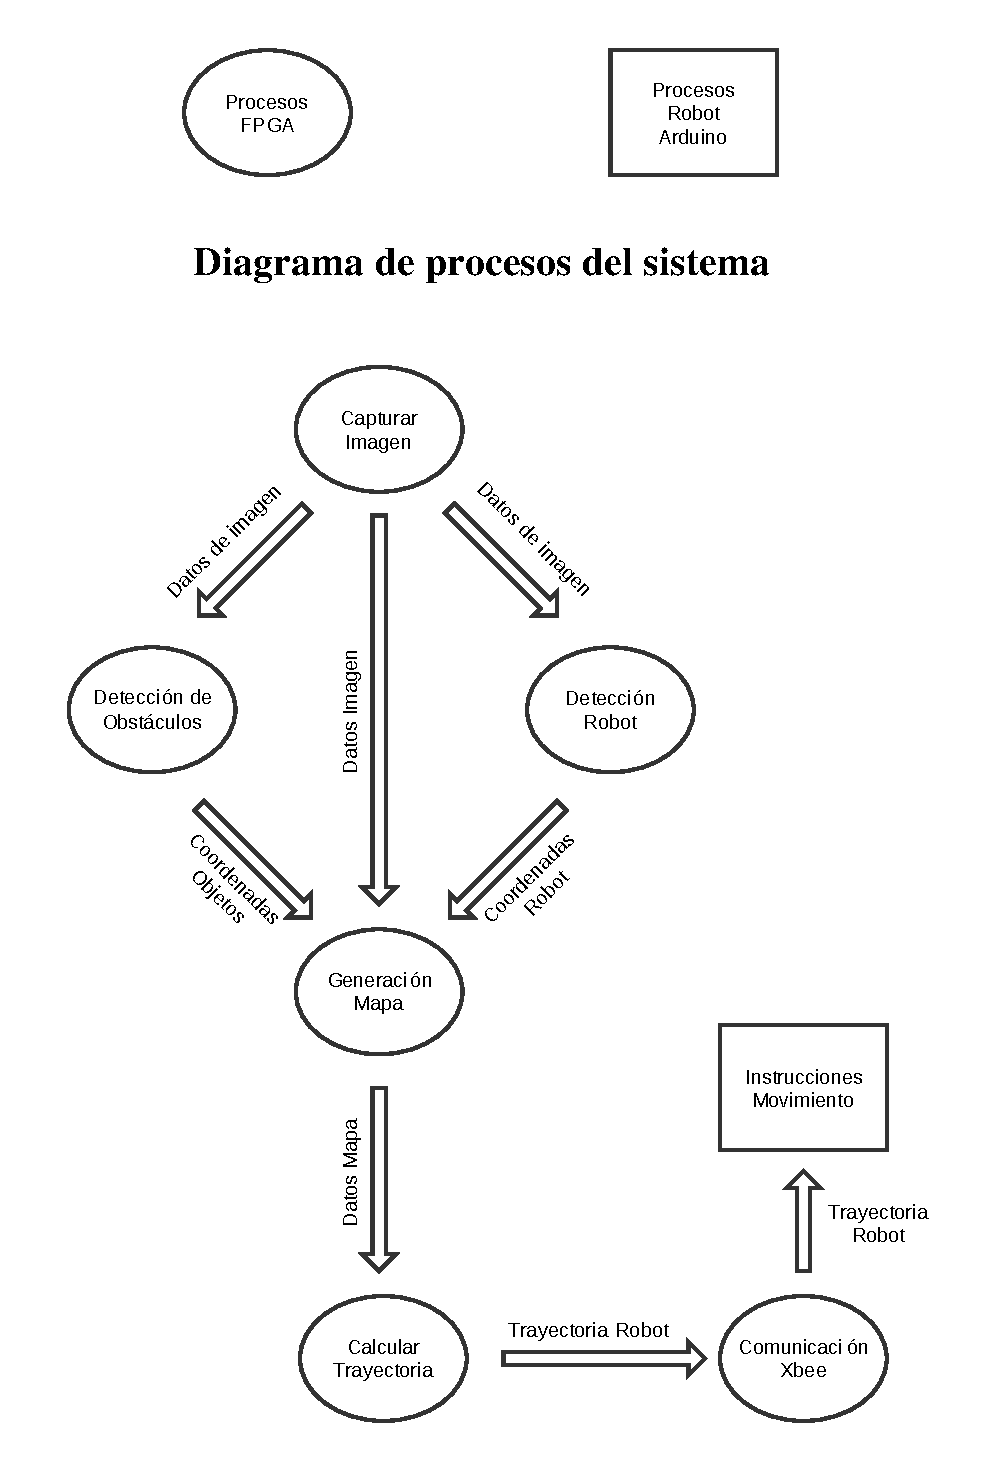
\includegraphics[height=0.873\textwidth]{procesosDelSistema}
\caption{Diagrama de procesos del sistema.}
\label{fig:DiagramaProcesos}
\end{figure}

%%HECHO-NOTA 2
% En la figura 1 en lugar de poner Detección de borde ponerr Detección de Obstáculos


\section{TECNOLOGÍA ESPECÍFICA / INTENSIFICACIÓN / ITINERARIO CURSADO POR EL ALUMNO}

\begin{table}[hp]
  \centering
  \caption{Tecnología Específica cursada por el alumno}
  \label{tab:tec-especifica}

  \zebrarows{1}
  \begin{tabular}{p{0.33\textwidth}}
    \textbf{Marcar la tecnología cursada} \\
    \hline
    Tecnologías de la Información \\
    Computación \\
    Ingeniería del Software \\
    \textcolor[rgb]{0.5,0.0,0.0}{Ingeniería de Computadores} \\
    \hline
  \end{tabular}
\end{table}


\clearpage

%En la segunda tabla, el alumno deberá justificar cómo \textbf{algunas}
%de las competencias específicas de la intensificación se aplicarán o
%tomarán forma en el TFG, \textbf{La relación de competencias por
%  intensificación se encuentran en el Anexo I al final de este
%  documento. }


\begin{table}[hp]
  \centering
  \caption{Justificación de las competencias específicas abordadas en el TFG}
  \label{tab:competencias}

  \zebrarows{1}
  \begin{tabular}{p{0.36\linewidth}p{0.58\linewidth}}
    \textbf{Competencia} & \textbf{Justificación} \\
    \hline
    Capacidad de diseñar y construir sistemas digitales, incluyendo computadores, sistemas basados en microprocesador y sistemas de comunicaciones. & Debido a que voy utilizar un vehículo (dirigido por Arduino), el cual, se va a comunicar mediante un módulo XBEE con la placa Xillinx Zedboard. Estoy desarrollando un nuevo sistema digital, formado por distinto hardware. \\
    Capacidad de desarrollar procesadores específicos y sistemas empotrados, así como desarrollar y optimizar el software de dichos sistemas & Dado que voy a embeber el algoritmo de procesamiento de imágenes en el hardware de la placa Xillinx Zedboard, estoy desarrollando un programa específico para las características del hardware, por lo que a la vez estoy optimizando el código para poder llevar a cabo la ejecución por hardware.\\
    Capacidad de analizar y evaluar arquitecturas de computadores, incluyendo plataformas paralelas y distribuidas, así como desarrollar y optimizar software para las mismas & Debido a que voy a utilizar la placa Xillinx Zedboard por su gran potencial a la hora de realizar cálculos paralelos sin dependencias. Estoy teniendo en cuenta las características del hardware, para poder exprimir todo su potencial, a la hora de mostrar resultados en tiempo real.\\
    Capacidad de diseñar e implementar software de sistema y de comunicaciones. & Al utilizar un módulo para que la placa Arduino se comunique con la placa Xillinx Zedboard, por radio, estoy realizando un software para que esta comunicación se lleve a cabo.\\
    Capacidad de analizar, evaluar y seleccionar las plataformas hardware y software más adecuadas para el soporte de aplicaciones empotradas y de tiempo real & Cumplo esta competencia dado que utilizo la placa Xillinx Zedboard por su potencial en el cálculo de operaciones en paralelo (sin dependencias) para poder cubrir los requisitos necesarios que exige el procesamiento de una imagen, así como, el cálculo de una trayectoria, en tiempo real.\\
    Capacidad para comprender, aplicar y gestionar la garantía y seguridad de los sistemas informáticos. & Realizaremos un estudio sobre la comunicación realizada por el módulo XBee, tanto en la placa Xillinx Zedboard y Arduino, para evitar la pérdida de información.\\
    Capacidad para diseñar, desplegar, administrar y gestionar redes de computadores. & Dado que el robot de Arduino se comunica por radio con la placa Xillinx Zedboard, cumplo esta competencia, debido a la red de comunicación existente entre el módulo de Arduino y la placa Xillinx Zedboard.\\
    \hline
  \end{tabular}
\end{table}


\section{OBJETIVOS}

%El objetivo principal del proyecto es conseguir que un vehículo, motorizado, esquive en tiempo real una serie de objetos para llegar desde un origen a un destino. Para ello, primero tendremos que conseguir que nuestra cámara cenital, conectada a la placa Xillinx Zedboard, detecte los objetos (mediante un algoritmo de detección de bordes) y genere la trayectoria necesaria para poder alcanzar el destino.

El objetivo principal del proyecto es \textbf{conseguir que un vehículo motorizado esquive en tiempo real una serie de objetos para llegar desde un origen a un destino}. 

Para ello,dividiremos el proyecto en tres etapas u objetivos específicos.
\begin{itemize}
\item Detección de objetos y definición de trayectoria hasta el destino utilizando para ello una cámara cenital y la placa de desarrollo Zedboard de AVNET
\item Desarrollo del módulo de comunicaciones para enviar datos desde la placa Zedboard a la placa Arduino conectada al vehículo
\item Desarrollo de un sistema de control de movimientos para vehículo motorizado utilizando Arduino.
\end{itemize}
%primero tendremos que conseguir que nuestra cámara cenital, conectada a la placa Xillinx Zedboard, detecte los objetos utilizando diferentes algoritmos y genere la trayectoria necesaria para poder alcanzar el destino.

%Tras definir la trayectoria, mandaremos señales de movimiento a la placa Arduino del vehículo motorizado, para que vaya realizando los movimientos correspondientes hasta llegar al destino.

%Por lo comentado anteriormente, podemos dividir los objetivos del trabajo en tres etapas:

%\begin{itemize}
%\item Procesamiento de imágenes.
%\item Comunicación entre la placa Xillinx Zedboard y Arduino.
%\item Movimiento del vehículo.
%\end{itemize}

Cabe destacar que al orientar el proyecto a una ejecución en tiempo real, se tiene en cuenta que aparezcan nuevos objetos en el mapa, con los que habrá que generar una nueva trayectoria. 

La tecnología que hay hoy en día, tanto para algoritmos de detección de imágenes, así como, el hardware con el que llevaremos a cabo los cálculos, son totalmente válidos para llegar a conseguir los objetivos planteados. %Es tal mi convencimiento, que voy a pasar a valorar uno a uno los procesos mencionados en la figura de la introducción (véase Fig.~\ref{fig:DiagramaProcesos}).
A continuación se detallarán los procesos indicados en la figura \ref{fig:DiagramaProcesos}


\begin{itemize}
\item Proceso Capturar Imagen. En este proceso obtendremos las imágenes tomadas por la cámara conectada a la placa Xillinx Zedboard.
%\item Proceso Detección Borde. Mediante un algoritmo de detección de bordes generaremos los objetos que están presentes en la imagen.
\item Proceso Detección Obstáculos. Mediante el uso de algoritmo de detección de objetos detectaremos aquellos que están presentes en la imagen.
\item Proceso Detección vehiculo. Una vez detectados los objetos, según las características predefinidas del vehículo, detectaremos cuál de los objetos, inmersos en la imagen, es el vehículo.
\item Proceso Generación Mapa. Tras haber aplicado el algoritmo de detección de objetos, analizaremos la imagen para poder generar un mapa con las zonas por las que podrá pasar el vehículo.
\item Proceso Calcular Trayectoria. Con el mapa generado previamente de referencia, aplicaremos el algoritmo de búsqueda (en principio, A*) y generaremos la ruta por la que se desplazará el vehículo.
\item Proceso Comunicación Xbee. Una vez hemos calculado todos los datos necesarios para saber por dónde se tiene que mover el vehículo. Establecemos la comunicación entre la placa Xillinx Zedboard y la placa Arduino.
\item Proceso Instrucciones de Movimiento. La placa Arduino recibe las instrucciones de movimiento mediante el módulo Xbee y procede a realizar los movimientos recibidos.
\end{itemize}

%De acuerdo a la Introducción, el alumno deberá especificar cuál o cuáles son las hipótesis de trabajo de las que se parten, qué se pretende resolver, y en base a eso formular el objetivo principal del TFG.

%El objetivo principal deberá desglosarse en sub-objetivos parciales. Los sub-objetivos deberán describirse de forma breve y concisa.

%Como preámbulo a la formulación del objetivo parcial, el alumno deberá discutir sobre las limitaciones y condicionantes a tener en cuenta en el desarrollo del TFG (lenguaje de desarrollo, equipos, madurez de la tecnología, etc.).

%Del mismo modo, será recomendable incluir una lista preliminar de requisitos del sistema a construir.


\section{MÉTODO Y FASES DE TRABAJO}

Como metodología de trabajo, para cumplir los objetivos planteados, utilizaremos Scrum. 

Hemos concordado quedar todos los martes desde el día 9 de Febrero de 2016 hasta el día de la presentación del TFG, para ir marcando objetivos cada semana, y así llevar un control exhaustivo del avance del proyecto.

En lo referente al diseño hardware utilizaremos una metodología de desarrollo ágil.

Debido a que llevo un control semanal del proyecto, me permite establecer objetivos asequibles en ese periodo de tiempo, ya que, antes de continuar con otro objetivo, primero comprobamos si los objetivos planteados previamente se han cumplido.

Como herramienta de control de la documentación del código, para poder ir anotando descripciones de los cambios realizados, utilizo Doxygen.

%Como herramienta para documentar los cambios realizados en el proyecto, utilizo la descripción de las actualizaciones que realizo en el repositorio de GitHub. Dónde establezco los cambios que he introducido.

\section{MEDIOS QUE SE PRETENDEN UTILIZAR}

\subsection{Medios Hardware}

El hardware necesario para realizar el TFG sería el siguiente:

\begin{itemize}
\item Placa Arduino UNO R3 ATmega328. Placa con la que gestionaremos los movimientos a realizar del vehículo.
\item Chasis con motor y ruedas. Sobre el que montaremos la placa Arduino.
\item Controlador de motores doble puente H-L298: Necesitamos este controlador, ya que la placa Arduino no puede gestionar directamente motores de corriente contínua.
\item Módulo XBee y conector Xbee por MicroUSB. Ambos nos permitirán establecer una conexión entre la placa Xillinx Zedboard y el robot de arduino.
\item Batería LiPo 11,1V 2200mAh: Necesaria para alimentar la placa de Arduino.
\item Osciloscopio y Multímetro: Para comprobar el funcionamiento del prototipo hardware.
\item Xillinx Zedboard: Con la que realizaremos los cálculos necesarios para la detección de bordes de los objetos, así como, la generación del mapa y el cálculo de la trayectoria del vehículo.
\item Cámara Web cenital: Para tomar las imágenes a las que realizar el procesamiento.
\item Ordenador del laboratorio ARCO: Necesario para representar los datos generados por el proyecto.
\end{itemize}


\subsection{Medios Software}

%El alumno deberá describir los medios software (lenguajes, entornos de desarrollo, herramientas de gestión y planificación, etc.) que prevé serán necesarios para el desarrollo del proyecto

Para la realización del código, he decido utilizar el lenguaje C, debido a que hay una extensa documentación y me permite, mediante la herramienta Xilinx Vivado Design Suite Edition generar el código vhdl necesario para embeber el programa en el hardware.

Como entorno de desarrollo, para la programación en C, estoy utilizando VIM. Mientras que para generar el código necesario para el hardware, utilizaré Xilinx Vivado HLS.

Para guardar mis avances del proyecto, estoy utilizando el repositorio Github. El cual utilizo también para la documentación, ya que, utilizo como editor de texto Latex. El cual me permite guardar mi documentación en el repositorio como si tratara de código. Para la generación de la documentación del código se utilizará Doxygen.

%%HECHO-NOTA3:    PARA LA GENERACION DE LA DOCUMENTACIÓN DEL CODIGO USAREMOS DOXYGEN

\section{Material Auxiliar de Estudio}

%En esta sección se incluirán todas las referencias bibliográficas, ordenadas alfabéticamente por el primer apellido del primer autor, de las obras de las cuales se haya realizado alguna cita en los apartados anteriores. Las referencias deberán contener datos básicos como nombre y apellidos de los autores, título de la obra, evento al que pertenece, páginas, fecha y lugar de celebración (si se tratara de artículos de congreso), ISBN, editorial y ciudad (si se tratara de libro), nombre de revista, páginas, volumen y número (si se tratara de revista), etc.

%Se empleará un formato de referencia reconocido en el ámbito académico como ACM\footnote{http://www.acm.org/sigs/publications/proceedings-templates}\footnote{http://www.cs.ucy.ac.cy/\~{}chryssis/specs/ACM-refguide.pdf}.301 Otros formatos aconsejables son, por ejemplo, IEEE, AMA, APA y AMA.
%
%A continuación una sección de «Referencias» con ejemplos de referencias con formato ACM para:

\begin{itemize}
\item Material con ejemplos para saber manejar la herramienta Xilinx Vivado~\cite{Zynq}.
\item Material para aprender los algoritmos de procesamiento de imágenes necesarios incluidos en la librería OpenCV~\cite{Open}.
\item Ejemplo de implementación de algoritmo de detección de bordes en la placa Xillinx Zedboard~\cite{SobelZedboard}.
\item Ejemplo Algoritmo detección de bordes en lenguaje C.~\cite{Sobel}.
\item Plantilla Latex, del laboratorio de ARCO, para la realización del anteproyecto~\cite{Latex}.
\end{itemize}


\bibliographystyle{alpha}
\singlespacing
\bibliography{main}

%\section{CONTRATO DE PROPIEDAD INTELECTUAL (si lo hubiera)}
%
%\newpage
%\section*{ANEXO I: Descripción de Competencias por Intensificación o Tecnología
%Específica\footnote{Este anexo se deberá borrar y no deberá ser incluido en el documento de anteproyecto final}}
%
%\subsection*{Intensificación de Computación}
%
%\begin{itemize}
%\item Capacidad para tener un conocimiento profundo de los principios fundamentales y
%  modelos de la computación y saberlos aplicar para interpretar, seleccionar, valorar,
%  modelar, y crear nuevos conceptos, teorías, usos y desarrollos tecnológicos relacionados
%  con la informática.
%\item Capacidad para conocer los fundamentos teóricos de los lenguajes de programación y
%  las técnicas de procesamiento léxico, sintáctico y semántico asociadas, y saber
%  aplicarlas para la creación, diseño y procesamiento de lenguajes.
%\item Capacidad para evaluar la complejidad computacional de un problema, conocer
%  estrategias algorítmicas que puedan conducir a su resolución y recomendar, desarrollar e
%  implementar aquella que garantice el mejor rendimiento de acuerdo con los requisitos
%  establecidos.
%\item Capacidad para conocer los fundamentos, paradigmas y técnicas propias de los
%  sistemas inteligentes y analizar, diseñar y construir sistemas, servicios y aplicaciones
%  informáticas que utilicen dichas técnicas en cualquier ámbito de aplicación.
%\item Capacidad para adquirir, obtener, formalizar y representar el conocimiento humano en
%  una forma computable para la resolución de problemas mediante un sistema informático en
%  cualquier ámbito de aplicación, particularmente los relacionados con aspectos de
%  computación, percepción y actuación en ambientes entornos inteligentes.
%\item Capacidad para desarrollar y evaluar sistemas interactivos y de presentación de
%  información compleja y su aplicación a la resolución de problemas de diseño de
%  interacción persona computadora.
%\item Capacidad para conocer y desarrollar técnicas de aprendizaje computacional y diseñar
%  e implementar aplicaciones y sistemas que las utilicen, incluyendo las dedicadas a
%  extracción automática de información y conocimiento a partir de grandes volúmenes de
%  datos.
%\end{itemize}
%
%
%\subsection*{Intensificación de Ingeniería de Computadores}
%
%\begin{itemize}
%\item Capacidad de diseñar y construir sistemas digitales, incluyendo computadores,
%  sistemas basados en microprocesador y sistemas de comunicaciones.
%\item Capacidad de desarrollar procesadores específicos y sistemas empotrados, así como
%  desarrollar y optimizar el software de dichos sistemas.
%\item Capacidad de analizar y evaluar arquitecturas de computadores, incluyendo
%  plataformas paralelas y distribuidas, así como desarrollar y optimizar software para las
%  mismas.
%\item Capacidad de diseñar e implementar software de sistema y de comunicaciones.
%\item Capacidad de analizar, evaluar y seleccionar las plataformas hardware y software más
%  adecuadas para el soporte de aplicaciones empotradas y de tiempo real.
%\item Capacidad para comprender, aplicar y gestionar la garantía y seguridad de los sistemas informáticos.
%\item Capacidad para analizar, evaluar, seleccionar y configurar plataformas hardware para
%  el desarrollo y ejecución de aplicaciones y servicios informáticos.
%\item Capacidad para diseñar, desplegar, administrar y gestionar redes de computadores.
%\end{itemize}
%
%
%\subsection*{Intensificación de Ingeniería del Software}
%
%\begin{itemize}
%\item Capacidad para desarrollar, mantener y evaluar servicios y sistemas software que
%  satisfagan todos los requisitos del usuario y se comporten de forma fiable y eficiente,
%  sean asequibles de desarrollar y mantener y cumplan normas de calidad, aplicando las
%  teorías, principios, métodos y prácticas de la Ingeniería del Software.
%\item Capacidad para valorar las necesidades del cliente y especificar los requisitos
%  software para satisfacer estas necesidades, reconciliando objetivos en conflicto
%  mediante la búsqueda de compromisos aceptables dentro de las limitaciones derivadas del
%  coste, del tiempo, de la existencia de sistemas ya desarrollados y de las propias
%  organizaciones.
%\item Capacidad de dar solución a problemas de integración en función de las estrategias,
%  estándares y tecnologías disponibles.
%\item Capacidad de identificar y analizar problemas y diseñar, desarrollar, implementar,
%  verificar y documentar soluciones software sobre la base de un conocimiento adecuado de
%  las teorías, modelos y técnicas actuales.
%\item Capacidad de identificar, evaluar y gestionar los riesgos potenciales asociados que pudieran presentarse.
%\item Capacidad para diseñar soluciones apropiadas en uno o más dominios de aplicación
%  utilizando métodos de la ingeniería del software que integren aspectos éticos, sociales,
%  legales y económicos.
%\end{itemize}
%
%
%\subsection*{Intensificación de Tecnologías de la Información}
%
%\begin{itemize}
%\item Capacidad para comprender el entorno de una organización y sus necesidades en el
%  ámbito de las tecnologías de la información y las comunicaciones.
%\item Capacidad para seleccionar, diseñar, desplegar, integrar, evaluar, construir,
%  gestionar, explotar y mantener las tecnologías de hardware, software y redes, dentro de
%  los parámetros de coste y calidad adecuados.
%\item Capacidad para emplear metodologías centradas en el usuario y la organización para
%  el desarrollo, evaluación y gestión de aplicaciones y sistemas basados en tecnologías de
%  la información que aseguren la accesibilidad, ergonomía y usabilidad de los sistemas.
%\item Capacidad para seleccionar, diseñar, desplegar, integrar y gestionar redes e
%  infraestructuras de comunicaciones en una organización.
%\item Capacidad para seleccionar, desplegar, integrar y gestionar sistemas de información
%  que satisfagan las necesidades de la organización, con los criterios de coste y calidad
%  identificados.
%\item Capacidad de concebir sistemas, aplicaciones y servicios basados en tecnologías de
%  red, incluyendo Internet, web, comercio electrónico, multimedia, servicios interactivos
%  y computación móvil.
%\item Capacidad para comprender, aplicar y gestionar la garantía y seguridad de los sistemas informáticos.
%\end{itemize}

\end{document}


% Local Variables:
% coding: utf-8
% mode: flyspell
% ispell-local-dictionary: "castellano8"
% mode: latex
% End:
